\documentclass[tikz]{standalone}
\usetikzlibrary{arrows.meta}
\begin{document}

\begin{tikzpicture}[-latex, arrows={-Triangle[angle=20:5pt,scale=1.5]}, scale=1.5]
	\node (X) at (0,0) {\((X, \tau)\)};
	\node (Y) at (4,0) {\((Y, \sigma)\)};
	\node (W) at (2,-1.5) {\((W, \omega)\)};

	\draw (X) to node [above] {\(f\)} (Y);
	\draw (X) to node [below left] {\(g\)} (W);
	\draw (W) to node [below right] {\(h\)} (Y);
\end{tikzpicture}

\begin{tikzpicture}[-latex, arrows={-Triangle[angle=20:5pt,scale=1.5]}, scale=1.5]
	\node (X) at (0,0) {\((X, \tau)\)};
	\node (Y) at (4,0) {\((Y, \sigma)\)};
	\node (W) at (2,-1.5) {\((W, \omega)\)};
	\node (FX) at (2,1.5) {\((f[X] , \sigma _{f[X]})\)};

	\draw (X) to node [above] {\(f\)} (Y);
	\draw (X) to node [below left] {\(g\)} (W);
	\draw (W) to node [below right] {\(h\)} (Y);
	\draw (X) to node [above left] {\(f'\)} (FX);
	\draw (FX) to node [above right] {\(\iota\)} (Y);
\end{tikzpicture}

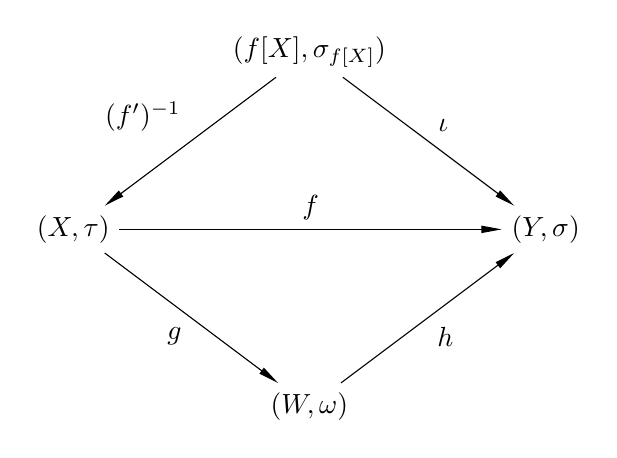
\begin{tikzpicture}[-latex, arrows={-Triangle[angle=20:5pt,scale=1.5]}, scale=1.5]
	\node (X) at (0,0) {\((X, \tau)\)};
	\node (Y) at (4,0) {\((Y, \sigma)\)};
	\node (W) at (2,-1.5) {\((W, \omega)\)};
	\node (FX) at (2,1.5) {\((f[X] , \sigma _{f[X]})\)};

	\draw (X) to node [above] {\(f\)} (Y);
	\draw (X) to node [below left] {\(g\)} (W);
	\draw (W) to node [below right] {\(h\)} (Y);
	\draw (FX) to node [above left] {\((f') ^ {-1}\)} (X);
	\draw (FX) to node [above right] {\(\iota\)} (Y);
\end{tikzpicture}

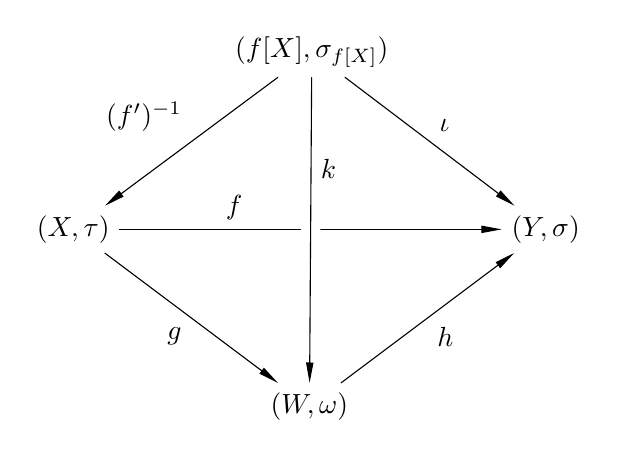
\begin{tikzpicture}[-latex, arrows={-Triangle[angle=20:5pt,scale=1.5]}, scale=1.5]
	\node (X) at (0,0) {\((X, \tau)\)};
	\node (Y) at (4,0) {\((Y, \sigma)\)};
	\node (W) at (2,-1.5) {\((W, \omega)\)};
	\node (FX) at (2.02,1.5) {\((f[X] , \sigma _{f[X]})\)};

	\draw (X) to node [pos=0.3,above] {\(f\)} (Y);
	\draw (X) to node [below left] {\(g\)} (W);
	\draw (W) to node [below right] {\(h\)} (Y);
	\draw (FX) to node [above left] {\((f') ^ {-1}\)} (X);
	\draw (FX) to node [above right] {\(\iota\)} (Y);
	\draw [line width=2.5mm,white] (FX) -- (W);
	\draw (FX) to node [pos=0.3, right] {\(k\)} (W);
\end{tikzpicture}

\begin{tikzpicture}[-latex, arrows={-Triangle[angle=20:5pt,scale=1.5]}, scale=1.5]
	\node (X) at (0,0) {\((X, \tau)\)};
	\node (Y) at (4,0) {\((Y, \sigma)\)};
	\node (W) at (2,-1.5) {\((W, \omega)\)};
	\node (FX) at (2.02,1.5) {\((f[X] , \sigma _{f[X]})\)};

	\draw (W) to node [below right] {\(h\)} (Y);
	\draw (FX) to node [above right] {\(\iota\)} (Y);
	\draw (X) to node [above left] {\(f'\)} (FX);
	\draw (FX) to node [pos=0.3, right] {\(k\)} (W);
\end{tikzpicture}

\begin{tikzpicture}[-latex, arrows={-Triangle[angle=20:5pt,scale=1.5]}, scale=1.5]
	\node [white] (X) at (0,0) {\((X, \tau)\)};
	\node (Y) at (4,0) {\((Y, \sigma)\)};
	\node (W) at (2,-1.5) {\((W, \omega)\)};
	\node (FX) at (2.02,1.5) {\((f[X] , \sigma _{f[X]})\)};

	\draw (W) to node [below right] {\(h\)} (Y);
	\draw (FX) to node [above right] {\(\iota\)} (Y);
	\draw (FX) to node [pos=0.3, right] {\(k\)} (W);
\end{tikzpicture}

\begin{tikzpicture}[-latex, arrows={-Triangle[angle=20:5pt,scale=1.5]}, scale=1.5]
	\node [white] (X) at (0,0) {\((X, \tau)\)};
	\node (Y) at (4,0) {\((Y, \sigma)\)};
	\node (W) at (2,-1.5) {\((W, \omega)\)};
	\node (FX) at (2.02,1.5) {\((f[X] , \sigma _{f[X]})\)};

	\draw (W) to node [below right] {\(h\)} (Y);
	\draw (FX) to node [above right] {\(\iota\)} (Y);
	\draw (W) to node [pos=0.7, right] {\(k ^ {-1}\)} (FX);
\end{tikzpicture}

\begin{tikzpicture}[-latex, arrows={-Triangle[angle=20:5pt,scale=1.5]}, scale=1.5]
	\node (X) at (0,0) {\((X, \tau)\)};
	\node (Y) at (4,0) {\((Y, \sigma)\)};
	\node (W) at (2,-1.5) {\((W, \omega)\)};
	\node (FX) at (2.02,1.5) {\((f[X] , \sigma _{f[X]})\)};

	\draw (X) to node [below left] {\(g\)} (W);
	\draw [{Triangle[angle=20:5pt,scale=1.5]}-{Triangle[angle=20:5pt,scale=1.5]}]
	(X) to node [above left] {\(f'\)} (FX);
	\draw [{Triangle[angle=20:5pt,scale=1.5]}-{Triangle[angle=20:5pt,scale=1.5]}]
	(FX) to node [right] {\(k\)}(W);
\end{tikzpicture}

\end{document}
